\documentclass[11pt,a4paper]{article}

\usepackage[margin=2.2cm]{geometry}
\usepackage[T1]{fontenc}
\usepackage{lmodern}
\usepackage{microtype}
\usepackage{amsmath}
\usepackage{graphicx}
\usepackage{booktabs}
\usepackage{tabularx}
\usepackage{array}
\usepackage{xcolor}
\usepackage{listings}
\usepackage{fvextra}
\usepackage{enumitem}
\usepackage{caption}
\usepackage{float}
\usepackage[hidelinks]{hyperref}

\graphicspath{{../results/charts/}{screenshots/}}
\setlist{itemsep=2pt, topsep=4pt}
\captionsetup{font=small, labelfont=bf}
\renewcommand{\arraystretch}{1.15}

\definecolor{codebg}{RGB}{248,248,250}
\definecolor{codekw}{RGB}{0,0,160}
\definecolor{codecm}{RGB}{90,120,90}
\lstset{
  language=Python, basicstyle=\ttfamily\footnotesize, backgroundcolor=\color{codebg},
  keywordstyle=\color{codekw}\bfseries, commentstyle=\color{codecm}\itshape,
  numbers=left, numberstyle=\tiny\color{gray}, frame=single, rulecolor=\color{gray!40},
  breaklines=true, showstringspaces=false, columns=fullflexible, xleftmargin=1.5em
}

\newcommand{\api}{http://10.1.75.53:3270}
% \input is not expandable, which breaks \bottomrule right after it in a table
\makeatletter\newcommand{\tabinput}[1]{\@@input #1 }\makeatother
\newcommand{\capture}[2]{%
  \subsubsection*{\texttt{#1}}
  \VerbatimInput[fontsize=\scriptsize, frame=single, rulecolor=\color{gray!40}, breaklines, breakanywhere]{#2}}

\title{\textbf{Assignment 7: Proximity Search API}\\[4pt]
\large Nearest locations by road distance within a circular radius}
\author{Rahul Raj \quad (12341680)\\ Computer Systems Design Lab}
\date{\today}

\begin{document}
\maketitle

\begin{center}
\begin{tabular}{ll}
\toprule
API & \texttt{\api/search/?lat=\&long=\&cat=\&rad=} \\
Demo page & \texttt{\api/} \\
Code & \texttt{Lab-Task/7.ProximitySearchAPI} in the CSD-Course repository \\
\bottomrule
\end{tabular}
\end{center}

\section*{Summary}

The API takes a position, a category and a radius, and returns the IDs of the 10 locations of that
category that are closest \emph{by road}, out of those lying inside the radius. The 10,000 locations form a
$100\times100$ grid of intersections, and \texttt{link.txt} says which neighbouring intersections are
connected by a road. About a quarter of the possible roads are missing, so a place that looks close on the
map can be a long drive away.

I treated it the way a ride-sharing app treats finding a nearby driver. The rider's position is snapped to
the nearest intersection, candidates are restricted to a radius, and they are ranked by how far you
actually have to drive. The road distances are computed with a breadth-first search (BFS) on the road graph
that stops as soon as the answer is known.

\begin{itemize}
  \item The results are the same as a brute-force Dijkstra search on 1,600 test queries (21 automated tests).
  \item In a simulation of the marking scheme on 2,000 random queries, ranking by road distance scores 100/100,
        while Euclidean and Manhattan ranking would score about 89.6 and 89.0.
  \item A query takes about 0.025\,ms inside the server and explores around 116 intersections. On a
        synthetic city with a million locations it still takes under 0.5\,ms.
\end{itemize}

% ---------------------------------------------------------------------------
\section{Problem}

The inputs are \texttt{lat}, \texttt{long}, \texttt{cat} and \texttt{rad}, and the output is a list of
10 location IDs. The assignment uses two different distances:

\begin{itemize}
  \item \textbf{Radius (straight line).} A location can only be returned if its Euclidean distance from
        $(\texttt{lat}, \texttt{long})$ is at most \texttt{rad}.
  \item \textbf{Closeness (along the grid).} Among those locations, ``closest'' means the shortest
        distance travelled along the roads. Roads only join neighbouring grid points (no diagonals), and
        some of them are missing.
\end{itemize}

Two consequences matter for the algorithm. A location inside the circle can be far away by road, and the
shortest road to a location inside the circle can go outside the circle and come back in.

% ---------------------------------------------------------------------------
\section{Data}

\subsection{Locations and roads}

\begin{table}[H]
\centering
\begin{tabularx}{0.92\textwidth}{>{\raggedright\arraybackslash}p{6cm}X}
\toprule
\textbf{Property} & \textbf{Value} \\
\midrule
\tabinput{tables/dataset.tex}
\bottomrule
\end{tabularx}
\caption{The dataset and the road network (from \texttt{scripts/analyze.py}).}
\end{table}

The locations form an exact grid. Location IDs follow the rule
$\text{ID} = 100\cdot\text{row} + \text{col} + 1$, where $\text{row} = 99\cdot\text{lat}$ and
$\text{col} = 99\cdot\text{long}$. So I can turn coordinates into an array index directly, with no lookup
table.

Each line of \texttt{link.txt} has the form \texttt{long\_A lat\_A long\_B lat\_B}. All 14,800 lines join
two neighbouring points, no line is repeated, and in every line point A has the smaller coordinate. So each
road is written once in a fixed order, which means roads can be used in both directions. I also tried
reading the lines as one-way roads. Then most of the map becomes unreachable (from node 6890 only 112 nodes
can be reached), so that reading is not what was intended (see also Section~\ref{sec:compare}). As an
undirected graph the network is connected. It is a spanning tree (9,999 roads) plus 4,801 extra roads that
form loops, and it has 111 dead ends.

\subsection{How much the missing roads matter}

\begin{figure}[H]
\centering
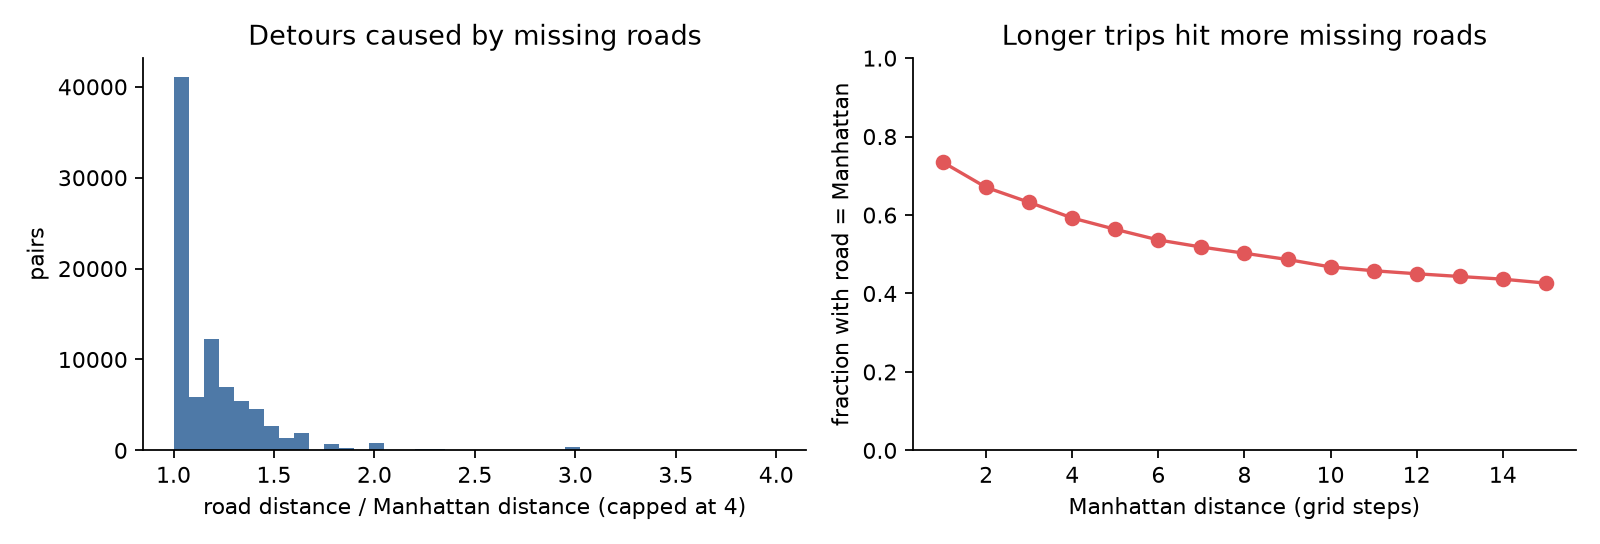
\includegraphics[width=\textwidth]{detour.png}
\caption{Left: road distance divided by Manhattan distance for all pairs at most 15 steps apart, from 200
random starting points. Right: fraction of pairs where the road distance equals the Manhattan distance.}
\end{figure}

\begin{table}[H]
\centering
\begin{tabular}{rrrrrr}
\toprule
Pairs & Road = Manhattan & Mean ratio & 90th pct & 99th pct & Max \\
\midrule
\tabinput{tables/detour.tex}
\bottomrule
\end{tabular}
\caption{Detour ratio (road distance / Manhattan distance).}
\end{table}

Only about half of the short trips can be driven along a shortest grid path. Longer trips are more likely to
run into a missing road, and the worst detour is 13 times the Manhattan distance.

% ---------------------------------------------------------------------------
\section{Choosing the distance}

\subsection{Options I considered}

\begin{table}[H]
\centering
\small
\begin{tabularx}{\textwidth}{>{\raggedright\arraybackslash}p{3.6cm}>{\raggedright\arraybackslash}p{3.6cm}X}
\toprule
\textbf{Distance} & \textbf{Models} & \textbf{Decision} \\
\midrule
Euclidean & flying in a straight line & used for the radius only; it ignores the roads \\
Manhattan & driving on a complete grid & only correct when no road on the way is missing \\
Chebyshev / 8 neighbours & diagonal moves & the assignment says there are no diagonal links \\
Haversine & distance on the Earth & the coordinates are a unit square, not degrees \\
\textbf{Shortest path on the road graph} & \textbf{driving on the actual roads} & \textbf{used for ranking} \\
Shortest path, one-way roads & directed streets & does not fit the data (Section~\ref{sec:compare}) \\
Travel time with turns or traffic & what real ride-sharing apps use & there is no speed, turn or traffic data \\
\bottomrule
\end{tabularx}
\caption{Candidate distance measures.}
\end{table}

Every road segment has the same length ($1/99$), so the shortest drive is the path with the fewest
segments. That is exactly what BFS finds, and Dijkstra's priority queue is not needed.

\subsection{Comparison with ride sharing}

A ride-sharing app matching a rider to a driver does roughly the same steps:
\begin{enumerate}
  \item \textbf{Map matching:} the rider's GPS position is snapped to the road network. Here, the query
        point is snapped to the nearest intersection.
  \item \textbf{Candidates by area:} drivers within some radius are taken from a spatial index. Here, the
        \texttt{rad} filter.
  \item \textbf{Ranking by driving distance:} candidates are ordered by route length or ETA, not by
        straight-line distance, since a driver on the other side of a river is not really close. Here, the
        BFS distance.
\end{enumerate}

\subsection{What each distance would score}\label{sec:compare}

I generated 2,000 random queries: half placed on a location and half anywhere, with radius between 0.08 and
0.35, and only queries with at least 10 valid answers were kept. For each one I computed the correct answer
with a separate Dijkstra search and scored every ranking the way the assignment does: one point for each
returned ID that is correct. IDs tied with the correct 10th place also count, since the TA said any tied
location is accepted.

\begin{figure}[H]
\centering
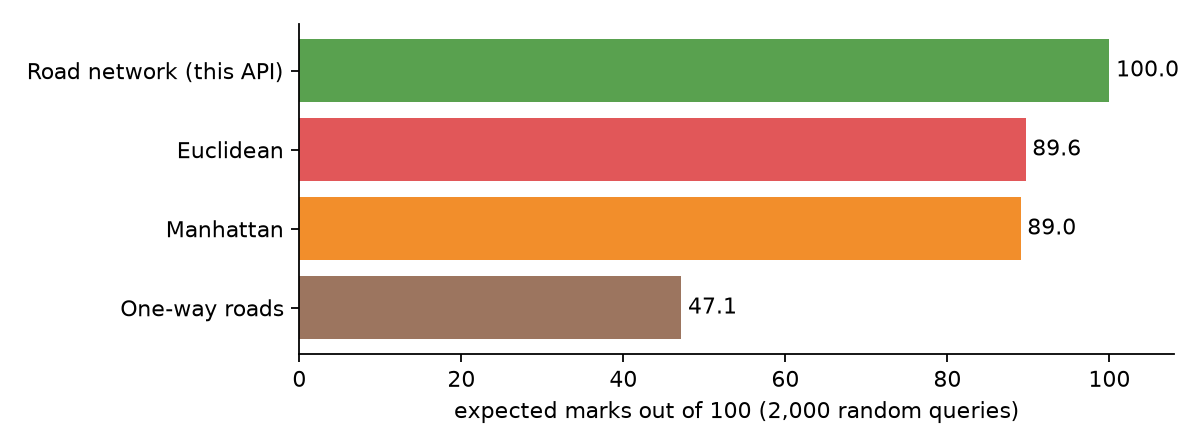
\includegraphics[width=0.8\textwidth]{metric_comparison.png}
\caption{Expected marks out of 100 for each ranking.}
\end{figure}

\begin{table}[H]
\centering
\begin{tabular}{lrrr}
\toprule
Ranking & Expected score / 100 & Queries fully correct & Worst query \\
\midrule
\tabinput{tables/metrics.tex}
\bottomrule
\end{tabular}
\caption{Simulated marks for 2,000 random queries.}
\end{table}

Euclidean and Manhattan get about 9 out of 10 IDs right on average, so at first they seem fine. But they get
the whole list right in less than a third of the queries, and in some places they miss most of it. The
one-way reading scores under half, which agrees with the roads being two-way.

\subsection{Example}

\begin{figure}[H]
\centering
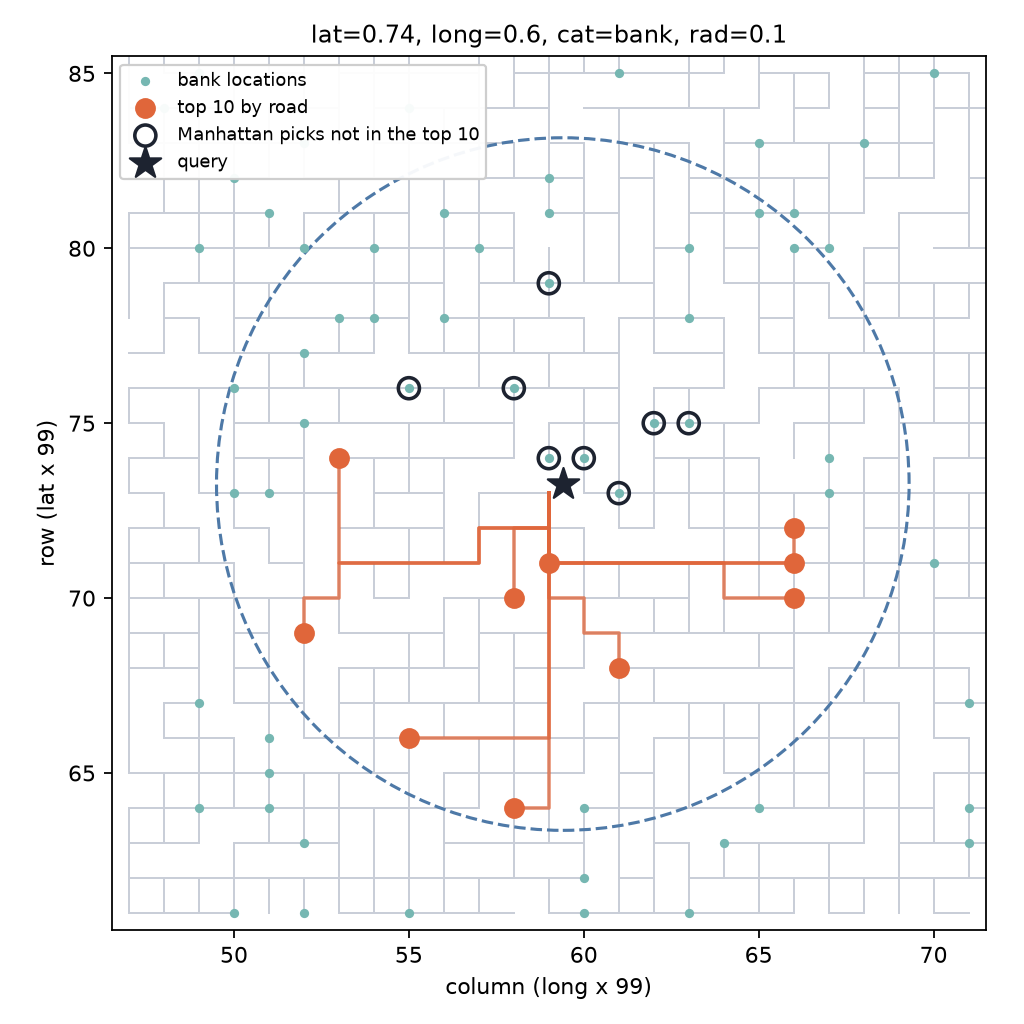
\includegraphics[width=0.72\textwidth]{example_query.png}
\caption{Query \texttt{lat=0.74, long=0.6, cat=bank, rad=0.1}. Grey lines are roads (gaps are missing
roads). Orange shows the 10 results and the routes to them. Circled banks are the ones Manhattan ranking
would return instead.}
\end{figure}

\begin{table}[H]
\centering
\small
\begin{tabular}{rrlrrr}
\toprule
Rank & ID & (lat, long) & Road steps & Manhattan steps & Straight line (steps) \\
\midrule
\tabinput{tables/example.tex}
\bottomrule
\end{tabular}
\caption{Results for the example query.}
\end{table}

The intersection nearest to the query has only one road, which goes south. Eight banks just north and east
of the query are 1 to 5 steps away in Manhattan distance, but they are far by road, so the road ranking
picks banks to the south and east instead. Manhattan ranking would get only 2 of the 10 right here.

% ---------------------------------------------------------------------------
\section{Algorithm}

\subsection{Data structures}

All of this is built once when the server starts, which takes about 25\,ms.
\begin{itemize}
  \item \texttt{adj[v]}: the neighbours of each node (14,800 roads, so 29,600 entries). The node number is
        $100\cdot\text{row}+\text{col}$, so a coordinate gives its node directly.
  \item \texttt{ids}, \texttt{lat}, \texttt{lon}, \texttt{cat}: plain lists indexed by node.
  \item For each category, numpy arrays with the coordinates of its 1,250 locations. These make it quick to
        count how many of them are inside the circle.
\end{itemize}

\subsection{BFS with early stopping}

\lstinputlisting[firstline=55, lastline=97, firstnumber=55]{../app/search.py}

The search works like this:
\begin{enumerate}
  \item Snap the query to its nearest node $s$ and count $T = \min(10, \text{locations inside the circle})$.
  \item Run BFS from $s$. When a node of the right category inside the circle is reached, add it to the
        results.
  \item When the $T$-th result is found, remember its distance $d_T$. Keep going until BFS reaches a
        node farther than $d_T$, then stop.
  \item Sort the results by (road distance, straight-line distance, ID) and return the first 10.
\end{enumerate}

\paragraph{Why stopping early is correct.} BFS takes nodes out of the queue in order of distance. Once it
reaches a node farther than $d_T$, every node not yet seen is at least that far, so none of them can be in
the top 10. Stopping after the whole $d_T$ level, not right at the 10th result, keeps every location tied
with the 10th, and the tie-break then chooses between them.

\paragraph{Why the circle does not limit the search.} The shortest road to a location inside the circle can
leave the circle, so nodes outside it still have to be expanded. The circle only decides which nodes count
as results. $T$ handles the case with fewer than 10 locations in the circle: once all of them are found the
search stops, instead of going through the whole map looking for ones that do not exist.

\paragraph{Unreachable locations.} Locations that cannot be reached are never returned, because BFS never
gets to them. The given network is connected, but the code does not depend on that.

\subsection{Complexity}

\begin{table}[H]
\centering
\begin{tabular}{ll}
\toprule
Step & Cost \\
\midrule
Count locations in the circle & $O(n/8)$ with numpy (1,250 points) \\
BFS & $O(V' + E')$ for the explored part only, $V' \approx 116$ on average \\
Sort results & $O(h \log h)$, $h \approx 10$--$15$ \\
Memory & $O(V + E)$, a few MB \\
\bottomrule
\end{tabular}
\end{table}

\paragraph{Alternatives.}
\begin{itemize}
  \item \textbf{Full Dijkstra for every query} (used as the reference in the tests) is about 130 times slower.
  \item \textbf{Precomputing all distances} ($10^4 \times 10^4$ values, about 200\,MB) is not needed at this
        speed.
  \item \textbf{A* to each candidate} would repeat work that a single BFS shares.
  \item \textbf{A k-d tree} would only speed up the radius count, which already takes microseconds.
\end{itemize}
For a large real road network with different road lengths, I would switch to Dijkstra or A*, or to
contraction hierarchies.

\subsection{Edge cases}

\begin{table}[H]
\centering
\small
\begin{tabularx}{\textwidth}{>{\raggedright\arraybackslash}p{3.2cm}>{\raggedright\arraybackslash}p{4.4cm}X}
\toprule
\textbf{Case} & \textbf{What the API does} & \textbf{Why} \\
\midrule
Query between intersections & snap to the nearest intersection (round each coordinate); points outside the
square go to the border & a car starts from the nearest intersection; for queries on a grid point this is exact \\
Location exactly on the circle & counted as inside, with a tolerance of $10^{-6}$ & the CSV rounds to 6
decimals, so a point exactly 3 steps away comes out about $5\cdot10^{-7}$ outside a radius of $3/99$ \\
Equal road distances & then straight-line distance, then ID & any tie is accepted; a fixed order makes results
repeatable \\
Category text & spaces trimmed, case ignored & \texttt{Hospital} and \texttt{hospital} are the same \\
Fewer than 10 valid & return the ones that exist & never return invalid IDs \\
\bottomrule
\end{tabularx}
\end{table}

% ---------------------------------------------------------------------------
\section{API}

\begin{table}[H]
\centering
\small
\begin{tabularx}{\textwidth}{>{\raggedright\arraybackslash}p{5.2cm}X}
\toprule
\textbf{Route} & \textbf{Description} \\
\midrule
\texttt{GET /search/?lat=\&long=\&cat=\&rad=} & returns \texttt{\{"ids": [...]\}} with 10 IDs, closest by road
first \\
\texttt{GET /search?...} & same handler; registered separately so there is no 307 redirect \\
\texttt{\&debug=1} & also returns road steps, straight-line and Manhattan distance, detour ratio and the full
route for each result \\
\texttt{GET /health} & number of locations and roads, categories, start-up time \\
\texttt{GET /} & demo page with a map (Figure~\ref{fig:demo}); \texttt{GET /docs} is the FastAPI docs page \\
\bottomrule
\end{tabularx}
\end{table}

Bad input returns HTTP 400 with a message naming the field: a missing parameter, a value that is not a
number, an unknown category, or a negative radius. CORS is enabled for GET requests.

\begin{figure}[H]
\centering
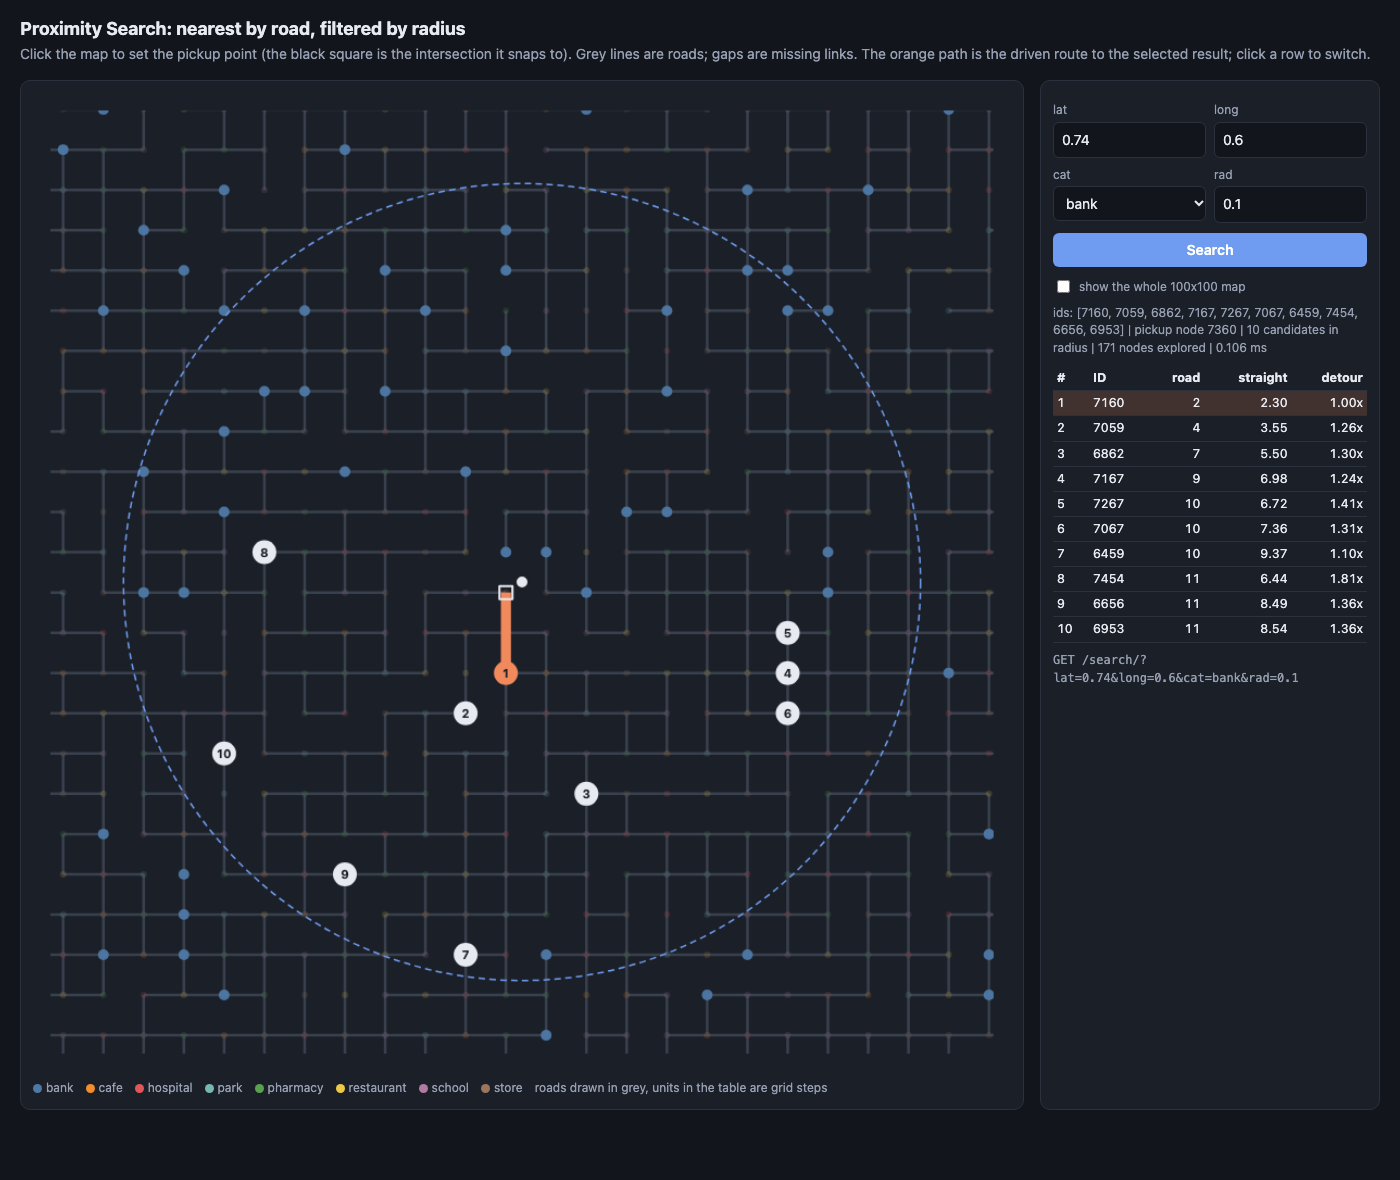
\includegraphics[width=\textwidth]{demo_map.png}
\caption{The demo page for the same query as the example above. The square marks the intersection the
query snaps to, and the orange line is the route to result 1.}
\label{fig:demo}
\end{figure}

% ---------------------------------------------------------------------------
\section{Testing}

\begin{itemize}
  \item \textbf{Against brute force:} for 1,600 random queries (half on grid points, radius from 0.02 to 2,
        all categories) the BFS gives exactly the same list, in the same order, as Dijkstra to all 10,000
        nodes followed by a sort.
  \item \textbf{Small hand-made networks:} a $3\times3$ grid with one missing road checks the exact order
        of the detours and the tie-break. A grid where some places cannot be reached checks that they are
        not returned. A diagonal link in the input is rejected.
  \item \textbf{Edge cases:} a point exactly on the circle, the corner of the map, points outside the map,
        always 10 results when 10 exist, every result inside the circle and of the right category, and
        Manhattan distances when there is no link file.
  \item \textbf{API:} route and parameter names, response format, no redirect without the slash,
        category case, the routes in debug output, and 400 for bad input.
\end{itemize}

\capture{01\_tests.txt}{terminal_captures/01_tests.txt}
\capture{02\_curl\_public.txt}{terminal_captures/02_curl_public.txt}

% ---------------------------------------------------------------------------
\section{Performance}

\subsection{Search time}

\begin{table}[H]
\centering
\begin{tabular}{lrrrr}
\toprule
Method (10,000 locations) & p50 (ms) & p95 (ms) & p99 (ms) & Nodes explored \\
\midrule
\tabinput{tables/latency.tex}
\bottomrule
\end{tabular}
\caption{Time per query inside the server, 5,000 random queries.}
\end{table}

\subsection{Larger cities}

To check that the search time does not grow with the size of the map, I generated random cities the same
way \texttt{link.txt} looks: a random spanning tree plus extra roads up to 75\% of all possible roads, with
random categories. The radius was 12 grid steps every time.

\begin{table}[H]
\centering
\begin{tabular}{rrrrrr}
\toprule
Locations & Roads & Load (s) & p50 (ms) & p99 (ms) & Nodes explored \\
\midrule
\tabinput{tables/scaling.tex}
\bottomrule
\end{tabular}
\caption{Search time on synthetic cities.}
\end{table}

BFS explores roughly the same number of nodes at every size, because it only goes as far as the 10 closest
results. The small increase at one million comes from counting the locations in the circle, which is linear
in the number of locations of the category.

\subsection{Over HTTP}

\capture{03\_loadtest\_local.txt (laptop)}{terminal_captures/03_loadtest_local.txt}
\capture{03\_loadtest\_public.txt (deployed API)}{terminal_captures/03_loadtest_public.txt}

On the laptop a single client gets a response in about 0.6\,ms. With 32 clients the laptop handles over 600
requests per second; at that point the load generator running on the same machine is the bottleneck. Against
the deployed API (one CPU core, through the lab NAT) the median response time with one client is about 8\,ms,
which is mostly network delay, and 32 clients get around 380 requests per second. There were no errors in
any run. The handler is \texttt{async} because a search takes much less than a millisecond, so running it in
a thread pool would cost more than the search itself.

% ---------------------------------------------------------------------------
\section{Deployment}

The API runs on lab machine \texttt{stu78\_sys2} in \texttt{\textasciitilde/assignment7} on port 3000, which
the lab NAT forwards to \texttt{\api}. The lab machines have no internet access, no cron and no tmux, and
their Python cannot create a normal virtual environment because \texttt{ensurepip} is missing. So
\texttt{scripts/deploy.sh} does the following:
\begin{enumerate}
  \item downloads the Linux x86-64 wheels for Python 3.12 on the laptop, using the versions
        pinned in \texttt{requirements.txt};
  \item copies the code, the data and the wheels over SSH with \texttt{tar} (there is no rsync on the
        machines);
  \item creates a virtual environment with \texttt{-{}-without-pip -{}-system-site-packages}, and installs
        the wheels offline with the system's pip;
  \item starts a small loop script with \texttt{setsid nohup}. It restarts uvicorn if it exits, and keeps
        pid files so that \texttt{deploy.sh stop} and \texttt{deploy.sh status} work without
        \texttt{pkill}.
\end{enumerate}

\capture{04\_restart\_after\_kill.txt}{terminal_captures/04_restart_after_kill.txt}

% ---------------------------------------------------------------------------
\section{Limitations and future work}

\begin{itemize}
  \item \textbf{Road lengths and speeds:} if roads had different lengths or speed limits, BFS would be
        replaced by Dijkstra or A*, and the ranking would become an actual travel time.
  \item \textbf{One-way roads and turns:} the graph can be made directed, and turn costs can be added by
        splitting each intersection into one node per direction.
  \item \textbf{Traffic and closed roads:} road weights could be updated while the server is running. Since
        nothing is precomputed, a change would apply from the next query on.
  \item \textbf{Starting point:} instead of snapping to one intersection, the search could start from both
        ends of the road the rider is on, each with the remaining distance along that road.
\end{itemize}

\end{document}
